\newpage
\section{ Árboles de Decisión y Bosques Aleatorios}
\noindent Sea un vector aleatorio $\textbf{x}$ con $p$ los datos de entrada, e $Y$ la variable respuesta. Supóngase también que se toman $n$ observaciones obteniéndose parejas $(\textbf{x}_i,y_i)$. De esta manera, tenemos que las $\textbf{x}_i\in \mathbb{R}^p$.\\
Los métodos de árboles son un método divisivo, ya que tras aplicarlos, se obtiene una partición del espacio de observaciones $\mathbb{R}^p$ y luego en cada región del espacio se ajusta un modelo más simple, incluso una constante.\\
La ventaja de este tipo de métodos es que son fácilmente interpretables, ya que pueden ser representados mediante un diagrama de tipo árbol. De esta manera, pueden ser utilizados según Brown \textit{et.al.}\cite{Brown 2004} tanto para análisis exploratorio, detectando características de grandes cantidades de datos, como para tareas de regresión y clasificación. \\ 
Las  siguientes imágenes procedentes de \textit{Hastie et. al.}\cite{Hastie 2001} muestran el diagrama resultante tras dividir el espacio de observaciones mediante un árbol.

\begin{figure}[h]
 \centering
  \subfloat[División de $\mathbb{R}^p$]{
   \label{f:división}
    \includegraphics[width=0.4\textwidth]{Documentos Extra/Imagenes/Regiones árboles.png}}
  \subfloat[Diagrama resultante]{
   \label{f:diagrama arbol}
    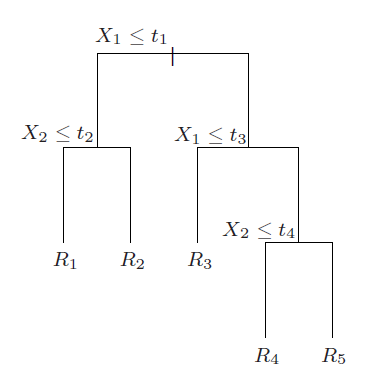
\includegraphics[width=0.4\textwidth]{Documentos Extra/Imagenes/Diagrama de arbol.png}}
 \caption{Representación de la división de $\mathbb{R}^p$ y el diagrama de árbol resultante}
 \label{f:MARC1}
\end{figure}

\noindent Otra ventaja de este tipo de métodos es que permite trabajar con conjuntos de datos en los que se estudian más variables en comparación de las observaciones, es decir, $p > n$. Por ejemplo, el ejemplo que desarrollan \textit{Díaz-Uriarte y De Andrés} \cite{Diaz 2006}, en el que trabajan con un microarray genético. 

\subsection{Árboles de Regresión}
\noindent Sea un vector aleatorio $\textbf{x}$ de variables predictoras como antes y una variable $Y$ de respuesta. 
Supóngase que queremos dividir el espacio de observaciones en $M$ regiones, $R_1,\ldots R_M$, se puede modelar en cada una de las regiones como la constante $c_m$. Por tanto teniendo en cuenta, la siguiente definición. 
\begin{equation}
\mathbf{1}_m(\textbf{x})=
\begin{cases}
0\quad& \text{si } x\notin R_m\\
1\quad& \text{si } x\in R_m\\
\end{cases}
\end{equation}
Es decir, la función $\mathbf{1}(\textbf{x})$ es la función característica de la región $R_m$, por tanto puede construirse el siguiente predictor:
\begin{equation}
f(\textbf{x})=\sum_{m=1}^M c_m \mathbf{1}_m(\textbf{x})
\end{equation}

\noindent Si se toma como criterio de ajuste los mínimos cuadrados obtendremos que $\hat{c}_m=ave(y_i|x_i\in R_m)$, ya que es la media condicional de la y sabiendo el valor de x. 

\noindent Para obtener las regiones se toma una variable $X_j$ y un valor de separación $s$, es decir, cada separación se puede identificar con una pareja $(j,s)$. 
Por ejemplo, supóngase una separación $(j,s)$ entonces se generan dos regiones del espacio de las observaciones $R_1, R_2$. 
\begin{equation}
R_1=\lbrace\textbf{x}|X_j\leq s\rbrace\quad R_2=\lbrace\textbf{x}|X_j > s\rbrace 
\end{equation}

\noindent Hay que establecer un criterio para elegir que separaciones se deben hacer en particular, para ello se utilizan los mínimos cuadrados:
\begin{equation}
\min_{j,s}\left[\min_{c_1}\sum_{x_i\in R_1}(y_i-c_1)^2+\min_{c_2}\sum_{x_i\in R_2}(y_i-c_2)^2\right]
\end{equation}

\noindent Es decir, teniendo en cuenta que se va a predecir el valor de la variable respuesta $y_i$ como una constante, la función anterior es la función $RSS$ 

\noindent Las mejores estimaciones de las constantes según el criterio de los mínimos cuadrados sería la media de las respuestas dentro de las regiones, es decir: 
\begin{equation}
\hat{c}_m=\dfrac{1}{n_m}\sum_{\textbf{x}_i\in R_m} y_i
\end{equation}

\noindent De esta manera, con estas estimaciones de las constantes de cada región, es posible encontrar la mejor división del espacio de observaciones. 

\noindent Se puede conseguir la mejor pareja $(j,s)$ fijando la $j$-ésima variable, encontrar el mejor valor $s$ para cada variable, de manera sencilla. 

\noindent El siguiente problema es controlar la complejidad del modelo, en particular, cuanto debe crecer el árbol, ya que un árbol demasiado grande  puede pecar de problemas de sobre ajuste. 

\noindent La estrategia más común es tener un criterio de parada, en particular hacer crecer un árbol grande $T_0$ y ``podarlo" cuando en los nodos terminales tenga menos de $5$ individuos según \textit{Díaz-Uriarte y De Andrés} \cite{Diaz 2006}, además este es el valor por defecto que otorga la librería de  \texttt{R, randomForest}. Si se hace más grande esto provoca que los árboles sean más pequeños. 

\begin{defi}
Llamaremos tamaño de un árbol $T$ y se denota por $|T|$ al número de nodos terminales, es decir, al número de regiones en las que se particiona el espacio de observaciones.
\end{defi}

\noindent Se puede entonces definir el error cuadrático medio de un nodo de un árbol de la siguiente manera:
\begin{equation}
Q_m(T)= \dfrac{1}{n_m}\sum_{\textbf{x}_i\in R_m}(y_i- \hat{c}_m)^2
\end{equation}

\noindent Con la anterior función y el concepto del tamaño del árbol, el cual está directamente relacionado con la complejidad del modelo, se puede establecer un criterio para un árbol que penalice la complejidad:
\begin{equation} \label{Eq Cost-Complexity}
C_{\alpha}(T)=\sum_{m=1}^{|T|}n_m Q_m(T) + \alpha|T|
\end{equation}

\noindent El valor de $\alpha$ es un parámetro que es elegido y su valor hace que se penalice más o menos la complejidad del modelo. A valores más altos, tendremos un modelo menos complejo y con $\alpha = 0$ es el modelo obtenido por mínimos cuadrados.

\noindent El objetivo es encontrar el árbol de menor tamaño para cada $\alpha$ que minimice la función \eqref{Eq Cost-Complexity}. Para ello se empieza con el árbol completo o con un árbol inicial $T_0$ e ir juntando los nodos que menor aumento provoquen sobre la función $\sum_{m=1}^{|T|}n_m Q_m(T)$, resultando en una secuencia de árboles entre los cuales se encuentra el que minimiza la función $C_{\alpha}(T)$ para un $\alpha $ determinado

 
\subsection{Árboles de Clasificación}
Gran parte de lo anterior se puede detallar de manera análoga a los árboles de regresión. 
\subsection{Bosques Aleatorios}

\noindent Los bosques aleatorios es una forma de utilizar varios árboles, de los cuales no se detallará el modo de construirlos. 

\noindent Sean $\textbf{x}, Y$ el vector de variables predictoras y la variable respuesta.